% Author: Izaak Neutelings (May 2022)
% https://github.com/IzaakWN/CodeSnippets/blob/master/LaTeX/TikZ/physics/tau_decay_matrix.py
% Inspiration:
%   https://texample.net/tikz/examples/pie-chart-color/
\documentclass[border=3pt,tikz]{standalone}
\usepackage{amsmath} % for \text
%\usepackage{mathabx} % for \widebar
\usepackage{bm} % for bold Greek letters via \bm
\usepackage[outline]{contour} % glow around text
\contourlength{0.25pt}

% STYLES
\usetikzlibrary{shapes} % for ellipse node
\usetikzlibrary{shadows.blur}
\colorlet{myred}{red!85!black!65}
\colorlet{mycyan}{blue!40!cyan!85!black!55}
\colorlet{myblue}{blue!70!cyan!85!black!55}
\colorlet{mydarkblue}{myblue!90!black!90}
\colorlet{mydarkerblue}{myblue!80!black!90}
\colorlet{mydarkestblue}{myblue!70!black!90}
\colorlet{mylightblue}{blue!50!cyan!80!black!45}
\colorlet{mypink}{magenta!95!red!100!black!72}
\colorlet{mypurple}{blue!50!red!90!black!70}
\colorlet{mydarkpurple}{blue!50!red!70!black!70}
\colorlet{mygreen}{green!60!black!75}
\colorlet{mylightgreen}{green!80!red!90!black!50}
\colorlet{myorange}{orange!95!black!70}
\colorlet{mybrown}{brown!80!orange!95!black!80}
\colorlet{myyellow}{yellow!80!orange!95!black!80}
\colorlet{mylightyellow}{yellow!80!orange!95!black!45}

\def\R{1} % default pie radius
\tikzstyle{pin}=[very thin,line cap=round]
\tikzset{
  slice/.style={fill=#1,draw=#1!80!black,line join=round,line width=0.4,
                blur shadow={shadow blur steps=20,shadow xshift=0.5,
                             shadow yshift=-1,shadow opacity=40}},
  slice/.default=myblue,
  pics/piechart/.style n args={2}{ % SIMPLE PIECHART 1
    code={
      \foreach \frac/\name/\col [
        count=\i,
        remember=\angb as \anga (initially #1), % start angle
        evaluate={\angm=\anga-\frac*1.8;  % middle angle
                  \angb=\anga-\frac*3.6;  % final angle
                  \exp=\R*max(0.02,0.2*(1-\frac/100)^8); % explode (radial shift)
                  \r=\exp+\R*max(0.5,(0.8-\frac/100));} % label radial positon
      ] in {#2}{ % loop over slices
        \coordinate (P\i) at (\angm:\exp+\R);
        \draw[slice=\col] % slice / circle sector
          (\angm:\exp) --++ (\anga:\R) arc(\anga:\angb:\R) -- cycle;
        \node[white,scale=0.9]
          at (\angm:\r) {\contour{\col!75!black}{\bm{$\frac\mathbf{\%}$}}};
        \node[\col!70!black,anchor=180+\angm,inner sep=4]
          at (P\i) {\bf\bm{$\name$}};
      }
    }
  },
  pics/piechart2/.style n args={2}{ % SIMPLE PIECHART 2
    code={
      \foreach \frac/\name/\col [
        remember=\angb as \anga (initially #1), % start angle
        evaluate={\angm=\anga+\frac*1.8;  % middle angle
                  \angb=\anga+\frac*3.6;  % final angle
                  \exp=\R*max(0.02,0.14*(1-\frac/100)^3); % explode (radial shift)
                  \r=\exp+\R*max(0.5,(1-\frac/100)^2);} % label radial positon
      ] in {#2}{ % loop over slices
        \message{^^J frac=\frac: anga=\anga -> angb=\angb}
        \draw[slice=\col] % slice / circle sector
          (\angm:\exp) --++ (\anga:\R) arc(\anga:\angb:\R) -- cycle;
        \ifdim \frac pt > 10pt % label inside slice
          \node[white,align=center]
            at (\angm:\r) {\boldlabel{$\name$}{\frac}};
        \else % label outside slice
          \node[\col!5!black,align=center,anchor=180+\angm,inner sep=3]
            at (\angm:\exp+\R) {\boldlabel{$\name$}{\frac}};
        \fi
      }
    }
  },
}

% MACROS
%\renewcommand\bar{\overline}
\newcommand\WW{\mathrm{WW}} %W^+W^-
\newcommand\ZZ{\mathrm{ZZ}}
\newcommand\TT{\tau\tau}
\newcommand\qbar{\bar{q}}
\newcommand\ttbar{\mathrm{t}\bar{\mathrm{t}}}
\newcommand\bbbar{\mathrm{b}\bar{\mathrm{b}}}
\newcommand\ccbar{\mathrm{c}\bar{\mathrm{c}}}
\newcommand\udbar{\mathrm{u}\bar{\mathrm{d}}}
\newcommand\csbar{\mathrm{c}\bar{\mathrm{s}}}
\newcommand\e{\mathrm{e}}
\newcommand\hp{\mathrm{h}^\pm}
\newcommand\hM{\mathrm{h}^\mp}
\newcommand\pz{\pi^0}
\newcommand\tauh{\tau_\mathrm{h}}
\newcommand\jets{\mathrm{jets}}
\newcommand\boldlabel[2]{\bf\bm{#1}\\[-1]\small\bm{$#2\mathbf{\%}$}}
\newcommand\boldlabeltiny[2]{\bf\bm{$#1$}\\[-2.5]\footnotesize\bm{$#2\mathbf{\%}$}}

\begin{document}


% TAU BRANCHING FRACTION - PIE CHART (SIMPLE)
% https://pdg.lbl.gov/2021/tables/rpp2021-sum-leptons.pdf
% https://arxiv.org/abs/2201.08458 (Table 1)
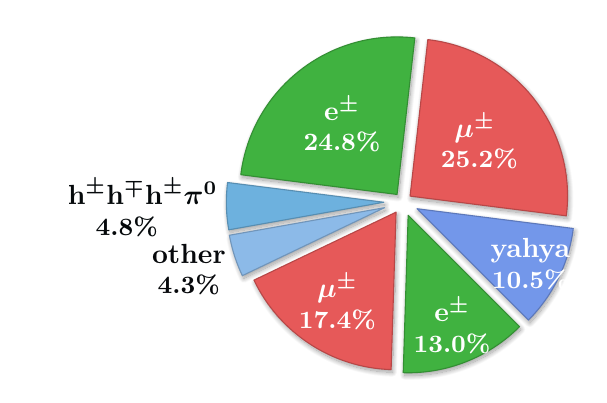
\begin{tikzpicture} %[scale=1.0,transform shape=false]
  %\message{^^JDitau pie chart}
  \draw pic[scale=2] {piechart2={-45}{
      10.5/\text{yahya}/myblue,
      25.2/\!\!\mu^\pm/myred,
      24.8/\e^\pm     /mygreen,
       4.8/\quad\hp\hM\hp\pz/mycyan!95!black,
       4.3/\text{other}     /mylightblue,
      17.4/\mu^\pm      /myred,
      13.0/\e^\pm           /mygreen%
  }};
  %\node[above,scale=1.2] at (0,1.8) {\bf\bm{$\tau$} lepton decay modes};
\end{tikzpicture}


% TAU BRANCHING FRACTION - PIE CHART (HADRONIC DECAY MODES)
% https://pdg.lbl.gov/2021/tables/rpp2021-sum-leptons.pdf
% https://arxiv.org/abs/2201.08458 (Table 1)
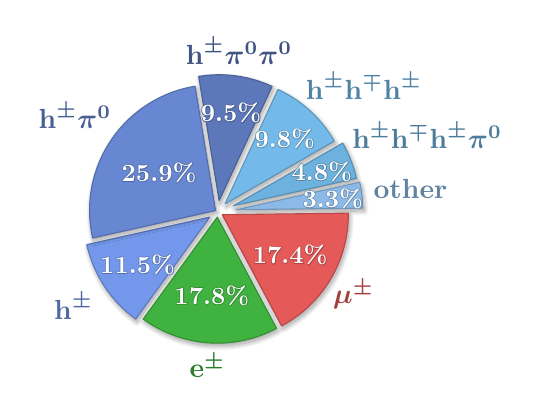
\begin{tikzpicture} %[scale=1.0,transform shape=false]
  %\message{^^JTau pie chart}
  \draw pic[scale=1.6] {piechart={-126}{
      11.5/\hp              /myblue,
      25.9/\hp\pz           /myblue!90!black,
       9.5/\hp\pz\pz        /myblue!80!black,
       9.8/\qquad\hp\hM\hp  /mycyan,
       4.8/\quad\hp\hM\hp\pz/mycyan!95!black,
       3.3/\text{other}     /mylightblue,
      17.4/\!\!\mu^\pm      /myred,
      17.8/\e^\pm           /mygreen%
  }};
%  \node[mycyan!70!black,anchor=-160] at (P4) {\bm{$\hp\hM\hp$}};
%  \node[mycyan!65!black,anchor=-160] at (P5) {\bm{$\hp\hM\hp\pz$}};
%  \node[above,scale=1.2] at (0,2.2) {\bf\bm{$\tau$} lepton decay modes};
\end{tikzpicture}


% DITAU BRANCHING FRACTION - PIE CHART
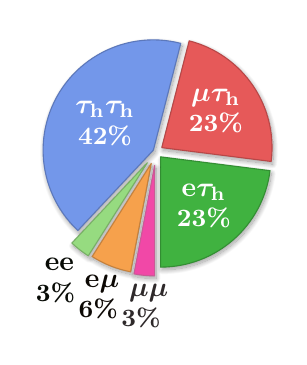
\begin{tikzpicture} %[scale=1,transform shape]
  \message{^^JDitau pie chart}
  \draw pic[scale=1.4] {piechart2={-90}{
    23/\e\tauh   /mygreen,
    23/\mu\tauh  /myred,
    42/\tauh\tauh/myblue,
     3/\;\e\e    /mylightgreen,
     6/\;\e\mu   /myorange,
     3/\;\;\mu\mu/mypink%
  }};
  %\node[above,scale=1.2] at (0,1.5) {\bf\bm{$\TT$} decay modes};
\end{tikzpicture}


% DITAU BRANCHING FRACTION - PIE CHART ALTERNATIVE
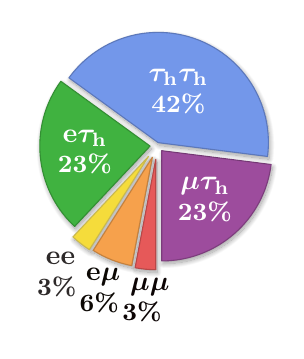
\begin{tikzpicture} %[scale=1.0,transform shape=false]
  \message{^^JDitau pie chart}
  \draw pic[scale=1.4] {piechart2={-90}{
    23/\mu\tauh  /mypurple,
    42/\tauh\tauh/myblue,
    23/\e\tauh   /mygreen,
     3/\;\e\e    /myyellow,
     6/\;\e\mu   /myorange,
     3/\;\;\mu\mu/myred%
  }};
  %\node[above,scale=1.2] at (0,1.5) {\bf \bf\bm{$\TT$} decay modes};
\end{tikzpicture}


% W BOSON / TOP QUARK MAIN BRANCHING FRACTION - PIE CHART
% https://pdg.lbl.gov/2021/tables/rpp2021-sum-quarks.pdf
% https://pdg.lbl.gov/2021/tables/rpp2021-sum-gauge-higgs-bosons.pdf
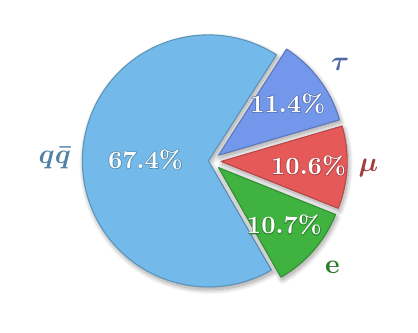
\begin{tikzpicture} %[scale=1.0,transform shape=false]
  \message{^^JW boson / top pie chart}
  \draw pic[scale=1.6] {piechart={-60}{
      67.4/q\qbar/mycyan,
      11.4/\tau  /myblue,
      10.6/\mu   /myred,
      10.7/\e    /mygreen%
  }};
  %\node[above,scale=1.2] at (0,1.6) {\bf Top decay modes};
\end{tikzpicture}


% W BOSON / TOP QUARK MAIN BRANCHING FRACTION - PIE CHART (SPLIT)
% https://pdg.lbl.gov/2021/tables/rpp2021-sum-quarks.pdf
% https://pdg.lbl.gov/2021/tables/rpp2021-sum-gauge-higgs-bosons.pdf
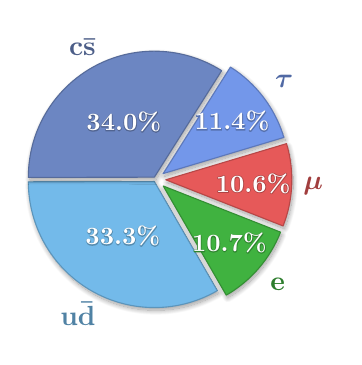
\begin{tikzpicture} %[scale=1.0,transform shape=false]
  \message{^^JW boson / top pie chart (split quarks)}
  \draw pic[scale=1.6] {piechart={-60}{
      33.3/\udbar/mycyan, %mylightblue,
      34.0/\csbar/mydarkerblue, %mycyan
      11.4/\tau  /myblue,
      10.6/\mu   /myred,
      10.7/\e    /mygreen%
  }};
  %\node[above,scale=1.2] at (0,1.7) {\bf Top decay modes};
\end{tikzpicture}


% TOP PAIR BRANCHING FRACTION - PIE CHART
% https://pdg.lbl.gov/2021/tables/rpp2021-sum-quarks.pdf
% https://pdg.lbl.gov/2021/tables/rpp2021-sum-gauge-higgs-bosons.pdf
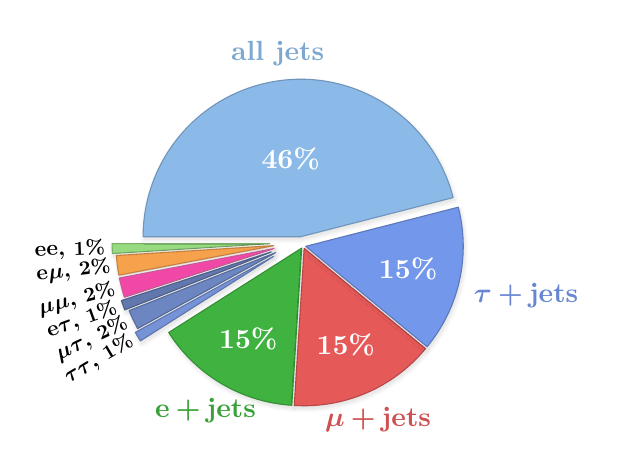
\begin{tikzpicture}[scale=2.0]
  \message{^^JWW or ttbar boson pie chart}
  %\node[above,scale=1.2] at (0,1.2) {\bf\bm{$\ttbar\to\bbbar\WW$} decay modes};
  
  % PIE CHART
  \def\angA{180} % initial angle
  \foreach \subgroup in { % loop over subgroup
     { 1/\e\e      /mylightgreen, % dileptonic decays
       2/\e\mu     /myorange,
       2/\mu\mu    /mypink,
       1/\e\tau    /mydarkestblue,
       2/\mu\tau   /mydarkerblue,
       1/\tau\tau  /mydarkblue},%
     {15/\e+\jets  /mygreen, % semileptonic decays
      15/\mu+\jets /myred,
      15/\tau+\jets/myblue},%
     {46/\text{all jets}/mylightblue}% % fully hadronic decays
  }{%
    \message{^^JSubgroup at angA=\angA}
    
    \def\ftot{0}
    \foreach \frac/\d/\d in \subgroup{
      \pgfmathparse{\ftot+\frac} \xdef\ftot{\pgfmathresult}
    }
    
    % MAKE SLICE FOR SUBGROUP
    \begin{scope}[shift={(\angA+\ftot*1.8:0.03*\R)}]
    \foreach \frac/\name/\col [
      remember=\angb as \anga (initially \angA), % start angle
      evaluate={\angm=\anga+\frac*1.8;  % middle angle
                \angb=\anga+\frac*3.6;  % final angle
                \exp=\R*0.2*(1-\frac/100)^15; % explode (radial shift)
                \r=\exp+\R*max(0.5,(1-\frac/100)^2.5);} % label radial positon
    ] in \subgroup{ % loop over subgroup
      \message{^^J  Slice at anga=\anga -> angb=\angb}
      \draw[slice=\col,shadow opacity=15] % slice / circle sector
        (\angm:\exp) --++ (\anga:\R) arc(\anga:\angb:\R) -- cycle;
      \ifdim \frac pt > 10pt % fraction inside slice
        \node[white]
          at (\angm:\r) {\bm{$\frac\mathbf{\%}$}};
        \node[\col!90!black,anchor=180+\angm,inner sep=5]
          at (\angm:\exp+\R) {\bf\bm{$\name$}};
      \else % fraction and label outside slice
        \node[black,align=center,anchor=0,rotate=180+\angm,inner sep=3,scale=0.8]
          at (\angm:\exp+\R) {\bf\bm{$\name$}, \small\bm{$\frac\mathbf{\%}$}};
      \fi
      \xdef\angA{\angb} % globally redefine \angA to last angle \angb
    }
    \end{scope}
    
  }
  
\end{tikzpicture}


% Z BOSON BRANCHING FRACTION - PIE CHART
% https://en.wikipedia.org/wiki/W_and_Z_bosons#Z0_boson
% https://pdg.lbl.gov/2021/tables/rpp2021-sum-gauge-higgs-bosons.pdf
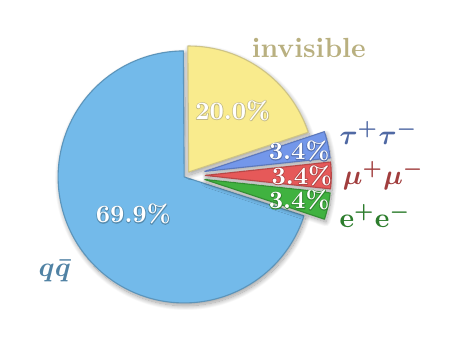
\begin{tikzpicture} %[scale=1.0,transform shape=false]
  \message{^^JZ boson pie chart}
  \draw pic[scale=1.6] {piechart={-18}{
      69.9/q\qbar      /mycyan,
      20.0/\qquad\text{invisible}/mylightyellow, %myorange
       3.4/\tau^+\tau^-/myblue,
       3.4/\mu^+\mu^-  /myred,
       3.4/\e^+\e^-    /mygreen%
  }};
  %\node[above,scale=1.2] at (0,1.7) {\bf Z boson decay modes};
\end{tikzpicture}


% Z BOSON BRANCHING FRACTION - PIE CHART (SPLIT)
% https://en.wikipedia.org/wiki/W_and_Z_bosons#Z0_boson
% https://pdg.lbl.gov/2021/tables/rpp2021-sum-gauge-higgs-bosons.pdf
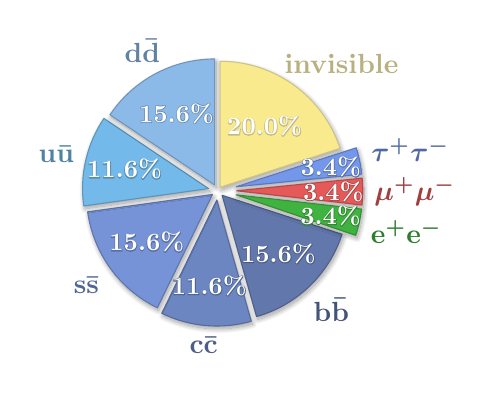
\begin{tikzpicture} %[scale=1.0,transform shape=false]
  \message{^^JZ boson pie chart}
  \draw pic[scale=1.6] {piechart={-18}{
      15.6/\bbbar/mydarkestblue, %mylightgreen
      11.6/\ccbar/mydarkerblue, %myorange,
      15.6/\mathrm{s\bar{s}}/mydarkblue,
      11.6/\mathrm{u\bar{u}}/mycyan,
      15.6/\mathrm{d\bar{d}}/mylightblue,
      20.0/\qquad\text{invisible}/mylightyellow, %myorange
       %6.7/\qquad\nu_\tau\nu_\tau/mylightyellow,
       %6.7/\qquad\nu_\mu\nu_\mu/mylightyellow,
       %6.7/\qquad\nu_\e\nu_\e/mylightyellow,
       3.4/\tau^+\tau^-/myblue,
       3.4/\mu^+\mu^-  /myred,
       3.4/\e^+\e^-    /mygreen%
  }};
  %\node[above,scale=1.2] at (0,1.9) {\bf Z boson decay modes};
\end{tikzpicture}


% HIGGS BRANCHING FRACTION - PIE CHART (MH = 125.1)
% https://twiki.cern.ch/twiki/bin/view/LHCPhysics/LHCHWG#Higgs_cross_sections_and_decay_b
% https://pdg.lbl.gov/2021/tables/rpp2021-sum-gauge-higgs-bosons.pdf
% other = 0.00202 = 1-(0.5807+0.2154+0.08179+0.06256+0.02883+0.02643+0.00227)
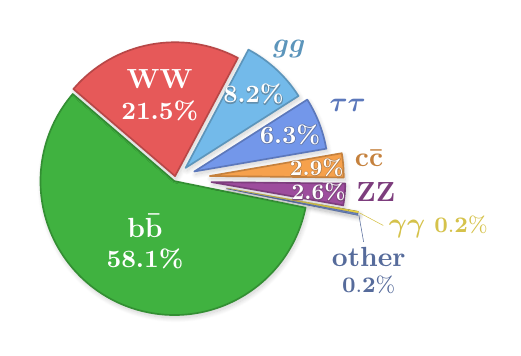
\begin{tikzpicture}[scale=1.7]
  \message{^^JHigss pie chart}
  \foreach \frac/\name/\col [
    count=\i,
    remember=\angb as \anga (initially -10), % start angle
    evaluate={\angm=\anga-\frac*1.8;  % middle angle
              \angb=\anga-\frac*3.6;  % final angle
              \exp=\R*max(0.02,0.4*(1-\frac/100)^15); % explode (radial shift)
              \r=\exp+\R*max(0.5,(0.83-\frac/100));} % label radial positon
  ] in { % loop over slices
       0.2/\gamma\gamma/myyellow,        % 0.00227
       0.2/other       /mydarkerblue,    % 0.00202
      %0.02/\mu\mu     /myblue!80!black, % 0.000217
      %0.02/Z\gamma    /myblue!80!black% % 0.001541
      58.1/\bbbar      /mygreen,  % 0.5807
      21.5/\WW         /myred,    % 0.2154
       8.2/gg          /mycyan,   % 0.08179
       6.3/\tau\tau    /myblue,   % 0.06256
       2.9/\ccbar      /myorange, % 0.02883
       2.6/\ZZ         /mypurple% % 0.02643
  }{
    \message{^^J frac=\frac: anga=\anga -> angb=\angb}
    \coordinate (P\i) at (\angm:\exp+\R);
    \draw[slice=\col,line width={\frac>2?0.6:0.2},shadow opacity=20] % slice / circle sector
      (\angm:\exp) --++ (\anga:\R) arc(\anga:\angb:\R) -- cycle;
    \ifdim \frac pt > 9pt % label inside slice
      \node[white,align=center]
        at (\angm:\r) {\boldlabel{$\name$}{\frac}};
    \else \ifdim \frac pt > 2pt % label inside slice, frac inside
      \node[white,scale={\frac>4?0.9:0.8}]
        at (\angm:\r) {\contour{\col!70!black!90}{\bm{$\frac\mathbf{\%}$}}};
      \node[\col!80!black,anchor=190+\angm,inner sep=4]
        at (P\i) {\bf\bm{$\name$}};
    %\else \ifdim \frac pt > 2pt % label & frac outside slice
    %  \node[\col!80!black,align=center,anchor=180+\angm,inner sep=3]
    %    at (P\i) {\bm{$\name$} \small$\mathbf{\frac\%}$}; %{\boldlabel{$\name$}{\frac}};
    %\else % pinned label
    %  \node[\col!80!black,align=center,pin={\angm-20:$\name$},inner sep=3]
    %    at (\angm:\exp+\R) {};
    \fi \fi %\fi
  }
  
  % MANUALLY PLACED LABELS
  \draw[pin,myyellow!85!black]
    (P1)++(-30:0.01) --++ (-28:0.2)
    node[anchor=178,inner sep=2]
      {\bm{$\gamma\gamma$} \footnotesize$\mathbf{0.2\%}$};
  \draw[pin,mydarkerblue!80!black]
    (P2)++(-40:0.01) --++ (-80:0.2)
    node[anchor=100,align=center,inner sep=2]
      {\bf other\\[-2.5]\footnotesize$\mathbf{0.2\%}$};
      %{\bm{$\mu\mu$}, \bf{$\mathrm{Z}\gamma$}, ...\\[-2.5]\footnotesize$\mathbf{0.2\%}$};
  
  %% TITLE
  %\node[above,scale=1.2] at (0,1.1) {\bf Higgs decay channels};
  
\end{tikzpicture}

  
% ENERGY DENSITY (Planck)
% https://doi.org/10.1051%2F0004-6361%2F201525830
% https://sci.esa.int/web/planck/-/51557-planck-new-cosmic-recipe
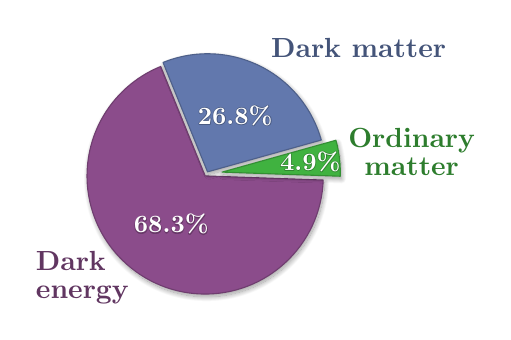
\begin{tikzpicture} %[scale=1.0,transform shape=false]
  \message{^^JEnergy density}
  \draw pic[scale=1.5] {piechart={-2}{
    68.3//mydarkpurple,
    26.8//mydarkestblue,
    4.9//mygreen%
  }};
  \node[anchor=5,inner sep=3,align=left,mydarkpurple!70!black]
    at (P1) {\bf Dark\\[-2]\bf energy};
  \node[anchor=-170,inner sep=4,mydarkestblue!70!black]
    at (P2) {\bf Dark matter};
  \node[anchor=185,inner sep=3,align=center,mygreen!70!black]
    at (P3) {\bf Ordinary\\[-2]\bf matter};
\end{tikzpicture}


\end{document}